\section{\Glsfmtfullpl{crna}}
\label{sec:circrnas}

\Glspl{crna} represent a novel class of \glspl{ncrna} that have garnered
significant attention in recent years due to their unique structural properties
and diverse biological functions.
Unlike linear \glspl{rna}, \glspl{crna} are characterized by a covalently
closed loop structure, which confers increased stability and resistance to
degradation by exonucleases, making them reliable biomarkers and potential
therapeutic targets in various
diseases\supercite{ma_circular_2020,hoque_exploring_2023,wilusz_circular_2017}.
Initially considered mere byproducts of \gls{mrna} splicing, \glspl{crna} have
now been recognized for their regulatory roles in gene expression, cellular
processes, and disease
mechanisms\supercite{cherubini_foxp1_2019,wilusz_360_2018}.

\subsection{Biogenesis}
\label{sec:circrna_biogenesis}
During standard gene expression, pre-\gls{mrna} is transcribed from \gls{dna}.
Splicing then removes introns and joins exons to produce mature
\gls{mrna}\supercite{black_mechanisms_2003}.
In conventional splicing, an upstream 5' splice site (donor) connects to a
downstream 3' splice site (acceptor), forming linear \gls{mrna}
(\cref{fig:circrna_splicing}a).
Conversely, for \glspl{crna}, a downstream 5' splice site connects to an
upstream 3' splice site in reverse order across at least one
exon\supercite{chen_expanding_2020}.
This backsplicing process is - just like conventional splicing - catalyzed by
the canonical spliceosome\supercite{starke_exon_2015} and results in a circular
\gls{rna} molecule (\cref{fig:circrna_splicing}b).

\subsubsection{Models}

\glspl{crna} are generated through two primary models of
biogenesis: the direct backsplicing model and the lariat-intermediate model.
The direct backsplicing model involves the covalent joining of a downstream 5'
splice site to an upstream 3' splice site, resulting in a circular structure
devoid of a \gls{polya} tail and 5' cap, which distinguishes \glspl{crna} from
linear \glspl{rna}\supercite{zhang_complementary_2014,ferreira_circular_2018}.
This model emphasizes the role of complementary sequences in the introns
flanking the exons, which facilitate the proximity of splice sites necessary
for backsplicing\supercite{zhang_complementary_2014,meganck_engineering_2021}.

In contrast, the lariat-intermediate model posits that \glspl{crna} can also
arise from lariat structures formed during canonical splicing.
In this scenario, introns are excised as lariats, and the remaining exons can
circularize, leading to \gls{crna}
formation\supercite{humphreys_ularcirc_2019,barrett_circular_2015}.
This model highlights the potential for exon skipping, where certain exons are
omitted during splicing, further contributing to \gls{crna}
diversity\supercite{sun_microarray_2020,barrett_circular_2015}.
Both models underscore the complexity of \gls{crna} biogenesis and the
interplay of various molecular mechanisms involved in their
formation\supercite{sharma_recent_2021}.

% TODO: Reference {fig:\gls{crna}_splicing}d

\subsubsection{Alternative splicing}
\label{sec:circrna_alternative_splicing}
In conventional splicing, introns are removed and exons are joined linearly.
However, in some cases, exons are skipped or introns are retained, leading to
alternative mature \gls{mrna} transcripts based on the same pre-\gls{mrna}.
This process is known as alternative splicing\supercite{nilsen_expansion_2010}.
Similarly, \glspl{crna} can be subject to alternative splicing.
This can result in the structures shown in \cref{fig:circrna_splicing}e and
\cref{fig:circrna_splicing}f.

\begin{figure}[H]
    \centering

    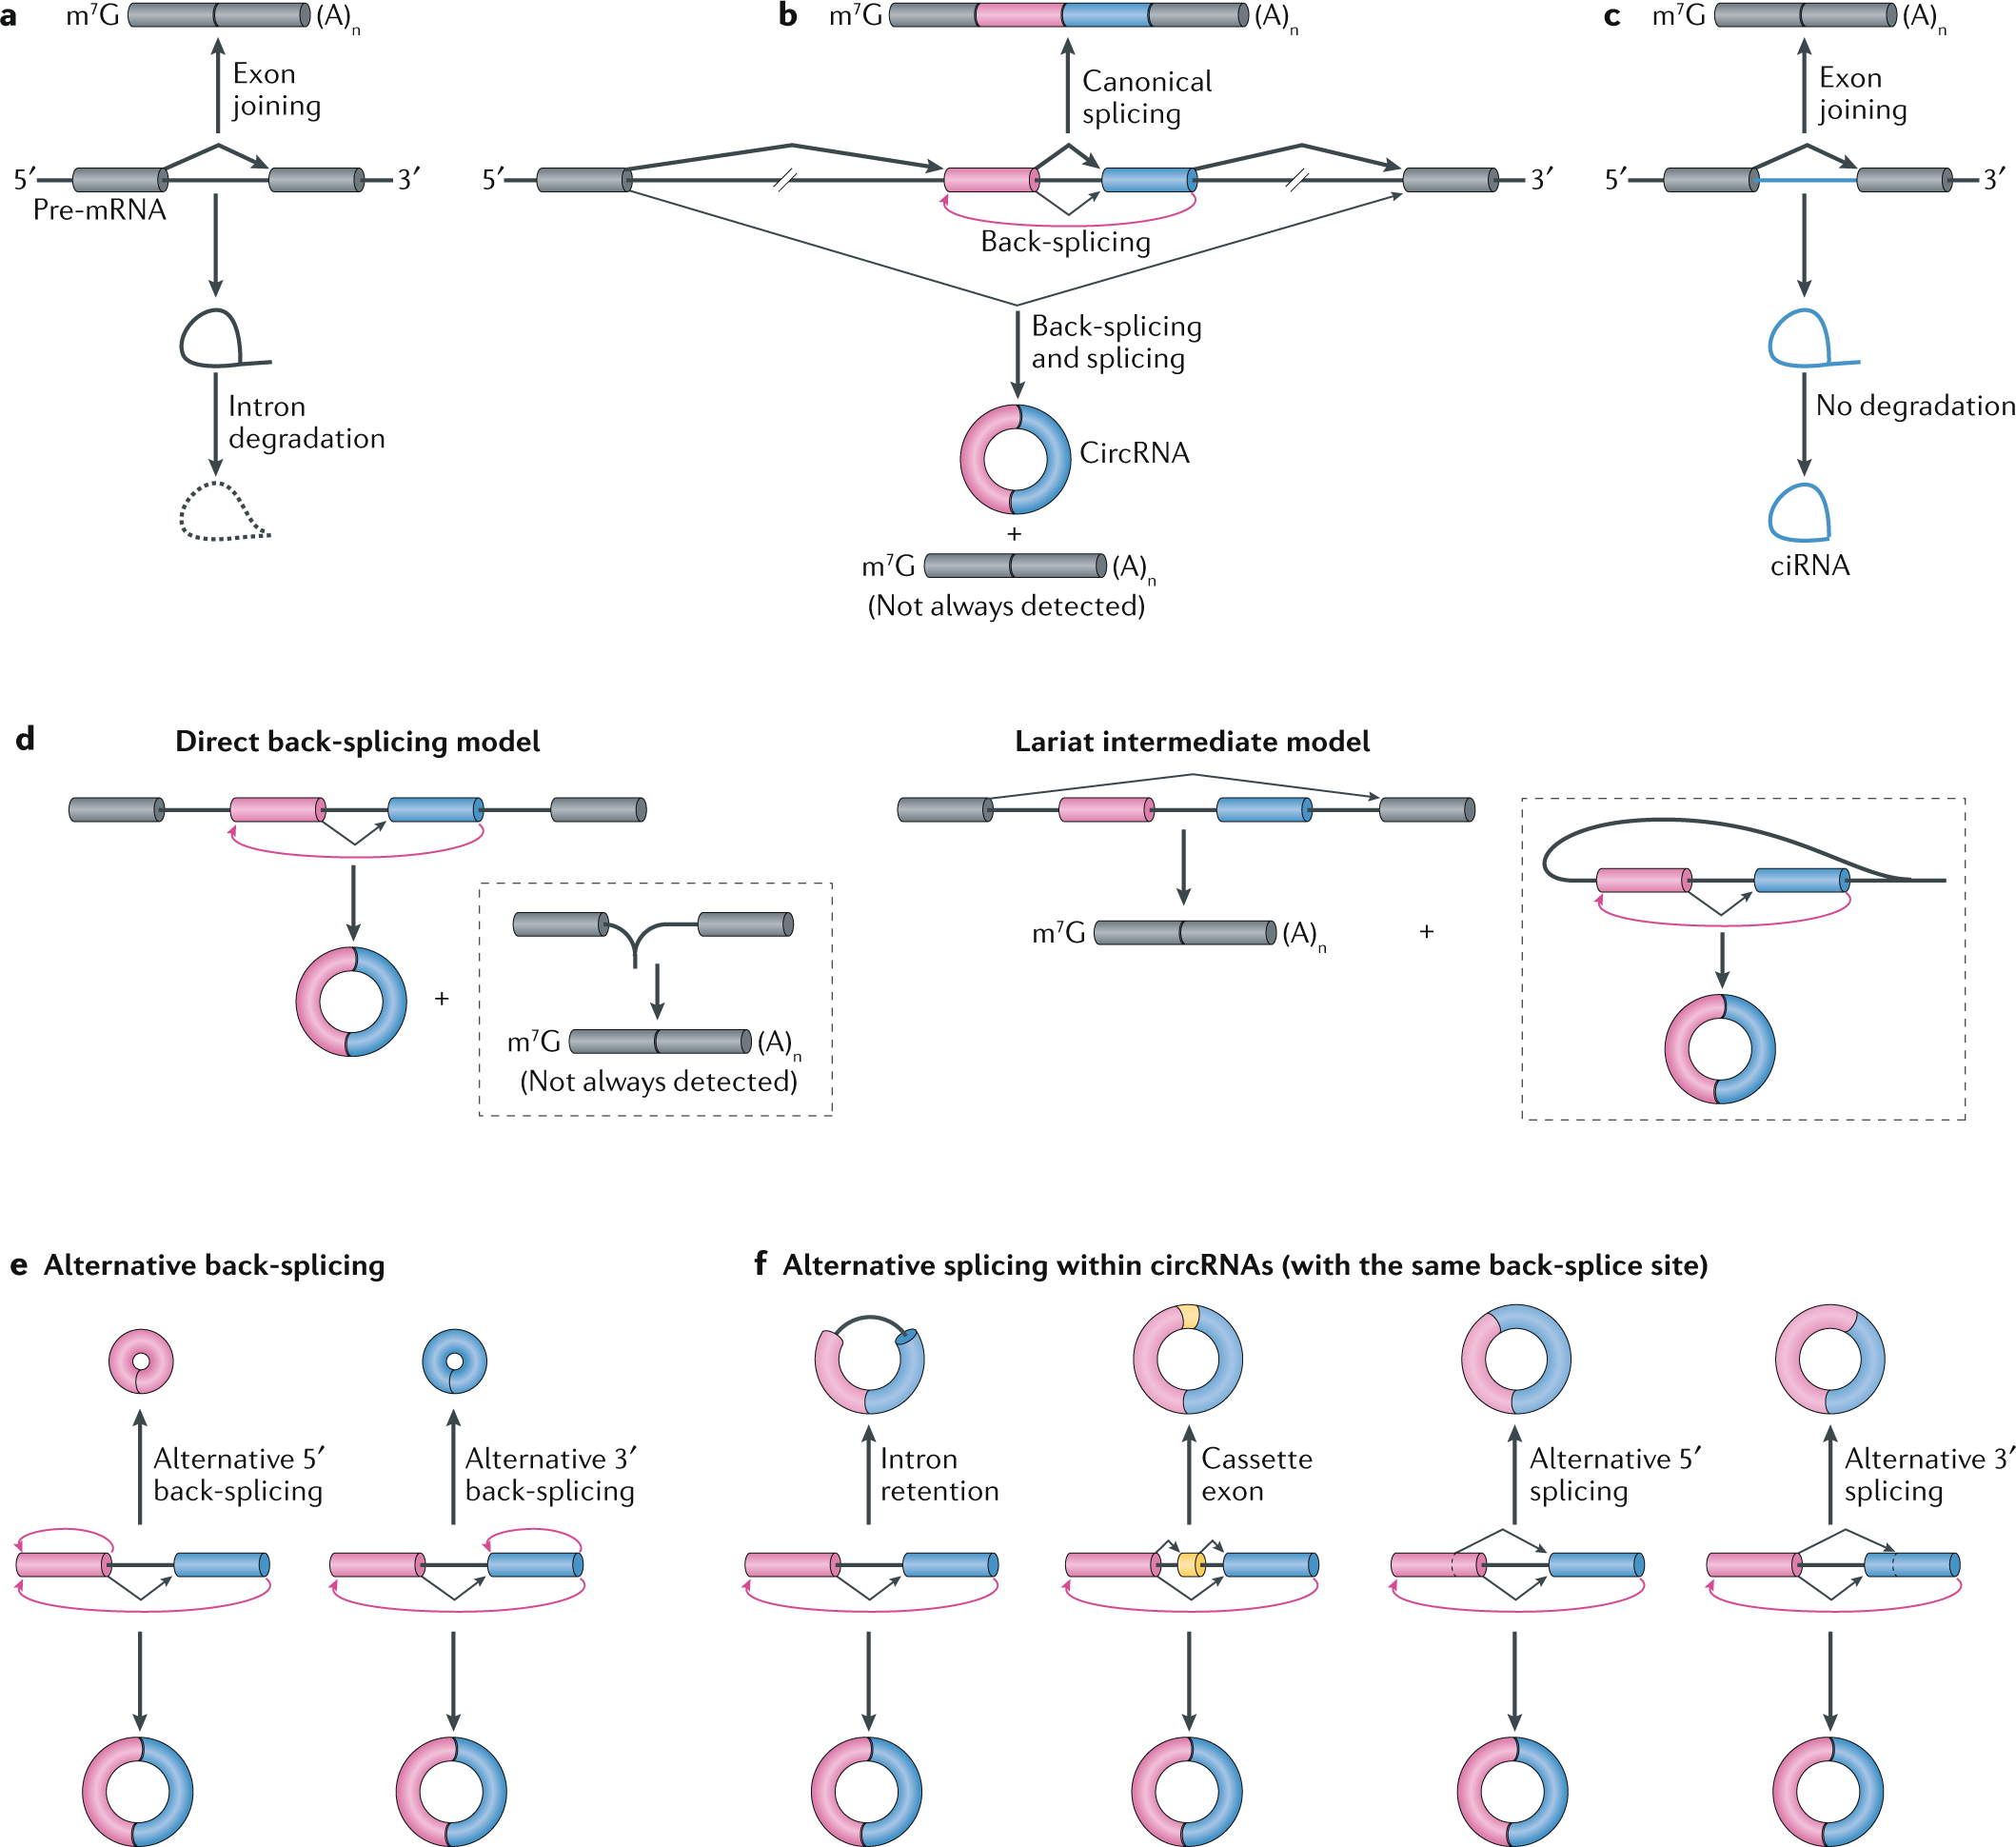
\includegraphics[width=\textwidth]{chapters/2_background/figures/circRNA-splicing.png}
    \caption{Splicing of \glspl{crna}} % TODO: Add detailed caption
    \label{fig:circrna_splicing}
\end{figure}

\subsection{\Glsfmtshort{crna} types}
\label{sec:circrna_types}

\Glspl{crna} can be classified into four main types based on their genomic
origins and structures.
Literature mostly uses a different nomenclature than the one presented here.

\begin{table}[ht]
    \centering
    \begin{tabular}{ccc}
        \hline
        Full name            & Thesis                & Literature
        \\ \hline
        \Glsfmtlong{e-crna}  & \glsfmtshort{e-crna}  & circRNA
        \\
        \Glsfmtlong{i-crna}  & \glsfmtshort{i-crna}  & ciRNA
        \\
        \Glsfmtlong{ei-crna} & \glsfmtshort{ei-crna} & EI-circRNA
        \\
        \Glsfmtlong{ig-crna} & \glsfmtshort{ig-crna} & Intergenic \gls{crna}
        \\ \hline
    \end{tabular}
    \caption{Comparison between the thesis' and literature's nomenclature for
        \glspl{crna}.
        The naming for \glspl{e-crna} is changed in order to avoid confusion with the
        overarching term \gls{crna}.
        The naming for \glspl{i-crna} is changed to be in line with the naming of
        \glspl{e-crna} and \glspl{ei-crna}.
    }
\end{table}

\paragraph{\Glsfmtfullpl{e-crna}} are the most prevalent type of \glspl{crna},
primarily formed from back-splicing of exons from protein-coding genes.
They are typically located in the cytoplasm and can function as sponges for
\glspl{mirna}, thereby modulating gene expression and influencing various
cellular processes, including tumorigenesis and cellular differentiation
(Bachmayr-Heyda et al., 2015; Wang et al., 2021).
\glspl{e-crna} have been shown to interact with \glspl{rbp}, which can
further regulate their stability and function (Zang et al., 2018).
Their abundance and stability make them potential biomarkers for various
diseases, including cancers (Li et al., 2021; Wang et al., 2021).

\paragraph{\Glsfmtfullpl{i-crna}}, on the other hand, are derived
from introns
and are predominantly localized in the nucleus.
They play a role in regulating the transcription of their parental genes and
are characterized by their constrained expression patterns (Ma et al., 2020;
Xie et al., 2023).
\gls{i-crna} are
believed to interact with components of the transcription machinery, thereby
influencing gene expression at the transcriptional level (Reddy et al., 2017).
The nuclear localization of \glspl{i-crna} suggests they may have distinct
regulatory functions compared to their \gls{e-crna} counterparts.

\paragraph{\Glsfmtfullpl{ei-crna}} are a hybrid form that
includes both
exonic and intronic sequences.
Like \glspl{i-crna}, \glspl{ei-crna} are also found in the nucleus and have
been implicated in the regulation of gene transcription.
They can enhance the expression of their parent genes by interacting with
\gls{pol2} and other transcription factors (Chen et al., 2022; Su, 2024).
This dual composition allows \glspl{ei-crna} to potentially serve as
intermediaries in the regulation of gene expression, bridging the functions of
both \glspl{e-crna} and \glspl{i-crna}.

\paragraph{\Glsfmtfullpl{ig-crna}} are formed from regions of
the
genome
that do not code for proteins and are often less characterized than the other
types.
Their functions remain largely unknown, but they are thought to contribute to
the regulatory networks within cells, possibly by interacting with other
\gls{rna} molecules or proteins (Li et al., 2021).
The study of \glspl{ig-crna} is still in its infancy, and further research is
needed to elucidate their roles in cellular processes.

\subsection{Biological functions}
\label{sec:circrna_functions}
\glspl{crna} have emerged as key players in various biological processes,
showcasing
a wide range of functions that contribute substantially to cellular regulation.

\subsubsection{\Glsfmtlong{mirna} sponging}
One of the most well-documented functions of \glspl{crna} is their ability to
act as \gls{mirna} sponges.
This mechanism involves the binding of \glspl{crna} to specific \glspl{mirna},
thereby preventing these \glspl{mirna} from interacting with their target
\glspl{mrna}.
For instance, the \gls{crna} CDR1as has been shown to contain over 60 binding
sites for miR-7, effectively sequestering it and allowing the expression of
miR-7 target genes to
increase\supercite{guo_expanded_2014,yuan_regulatory_2020}.
This \gls{cerna} activity is crucial in regulating gene expression and has been
implicated in various cancers, including gliomas and gynecological
cancers\supercite{dong_expression_2020,song_circular_2016}.
Additionally, \glspl{crna} such as circ-0000437 have been identified as sponges
for \glspl{mirna} involved in tumor progression, highlighting their potential
as therapeutic targets\supercite{li_peptide_2021,cui_circular_2022}.

\subsubsection{Protein interactions}
Beyond \gls{mirna} sponging, \glspl{crna} also participate in protein
interactions.
They can serve as scaffolds for \glspl{rbp}, influencing various cellular
processes, including transcription and
splicing\supercite{li_comprehensive_2017,qu_emerging_2017}.
For example, \glspl{crna} can recruit RBPs to specific genomic loci, thereby
modulating the transcriptional landscape of the
cell\supercite{li_comprehensive_2017}.
This interaction can lead to the regulation of gene expression at multiple
levels, further emphasizing the multifaceted roles of \glspl{crna} in cellular
biology\supercite{zhang_important_2024,he_targeting_2021}.
Moreover, some \glspl{crna} have been shown to interact with proteins that are
involved in signaling pathways, such as the Wnt/\textbeta{}-catenin pathway,
thereby influencing cellular proliferation and
differentiation\supercite{peng_novel_2021}.

\subsubsection{Translation into peptides}
In the canonical initiation of translation, ribosomes bind to the 5' cap of an
\gls{mrna} \supercite{hinnebusch_mechanism_2012}.
Because \glspl{crna} are circular and lack a 5' cap, they were long thought to
be non-coding \supercite{bao_regulatory_2019,greene_circular_2017}.
However, research has shown that \glspl{crna} with internal ribosome entry
sites can indeed be translated into proteins \supercite{chen_expanding_2020}:

\paragraph{\Glsfmtfullpl{ires}} In 1988, researchers discovered that certain
viral and cellular \glspl{mrna} contain sequences allowing ribosomes to
initiate translation without a 5' cap \supercite{pelletier_internal_1988,
    jang_segment_1988}.
These sequences are known as \gls{ires}.
In 1995, Chen and Sarnow demonstrated that artificially engineered \glspl{crna}
containing an \gls{ires} sequence are translated into peptides
\supercite{chen_initiation_1995}.
Later, it was found that some \glspl{crna} naturally possess \gls{ires}
sequences and can thus be translated into peptides
\supercite{chen_expanding_2020,legnini_circ-znf609_2017,pamudurti_translation_2017}.
A concrete example for an \gls{ires} is the consensus motif for
N\textsuperscript{6}-methyladenosine modification
\supercite{yang_extensive_2017}.

\paragraph{N\textsuperscript{6}-methyladenosine (m\textsuperscript{6}
    A)}  m\textsuperscript{6}A is the most abundant base modification in eukaryotic
\gls{rna} \supercite{yang_extensive_2017,li_pivotal_2014,wei_methylated_1975}.
% General introduction to m6A
Research has shown that m\textsuperscript{6}A modification can affect
localization, splicing, translation and degradation of \gls{rna} molecules
\supercite{yue_rna_2015,meyer_dynamic_2014}.
The effect of m\textsuperscript{6}A modification on translation is particularly
interesting, as it has been shown that m\textsuperscript{6}A modifications in
3' \glspl{utr} can enhance translation
efficiency\supercite{wang_n6-methyladenosine_2015}, while m\textsuperscript{6}A
modifications in 5' \glspl{utr} can promote cap-independent translation,
especially in heat shock stress\supercite{zhou_dynamic_2015,meyer_5_2015}.

% Build bridge to IRES-dependent mechanism
m\textsuperscript{6}
A modifications mostly occur in the consensus motif RRm\textsuperscript{6}ACH
(R = purine, H = non-guanine base)
\supercite{csepany_sequence_1990,harper_sequence_1990}, which has been found to
be enriched in \glspl{crna} \supercite{yang_extensive_2017}.
In \glspl{crna}, a single m\textsuperscript{6}A modification is often enough to
initiate translation\supercite{yang_extensive_2017}.

\subsection{Potential applications}
\label{sec:circrna_applications}
The unique properties of \glspl{crna}, such as their stability, abundance, and
specific expression patterns, make them attractive candidates for various
applications in the field of molecular biology and medicine.
Their potential uses include serving as biomarkers for disease diagnosis and
prognosis, therapeutic targets for drug development, and tools for gene
regulation and editing.

\subsubsection{Biomarkers}
One of the most compelling applications of \glspl{crna} lies in their potential
as biomarkers for cancer diagnosis and prognosis.
Studies have demonstrated that \glspl{crna} can serve as reliable indicators of
tumor progression and treatment response.
For instance, \glspl{crna} exhibit higher expression levels in certain cancers
compared to their linear counterparts, suggesting their utility in liquid
biopsies for non-invasive cancer
monitoring\supercite{bao_prognostic_2020,ren_construction_2017}.
Their stability in bodily fluids such as plasma and saliva further enhances
their applicability as biomarkers, as they are less prone to degradation than
traditional \gls{rna}
markers\supercite{bao_prognostic_2020,zhang_circular_2018}.
Specific \glspl{crna}, such as hsa\_circ\_0000190, have been correlated with
advanced stages of lung cancer, indicating their potential role in clinical
settings\supercite{luo_plasma_2020}.
Moreover, \glspl{crna} have been implicated in chemoresistance, providing
insights into treatment efficacy and patient
management\supercite{geng_function_2018,feng_functions_2019}.

Beyond their role in cancer, \glspl{crna} are also being explored in the
context of autoimmune diseases and neurological disorders.
For example, \glspl{crna} have been identified as novel biomarkers for
rheumatoid arthritis and multiple sclerosis, highlighting their versatility in
reflecting disease states beyond
oncology\supercite{ouyang_identification_2021,he_exosomal_2019}.
Their expression profiles in various tissues suggest that \glspl{crna} may play
a role in the pathophysiology of these conditions, potentially guiding
therapeutic strategies\supercite{mohammed_circular_2023}.

\subsubsection{Therapeutic targets}
In addition to their diagnostic potential, \glspl{crna} are being investigated
as therapeutic targets.
Their ability to modulate gene expression and interact with \glspl{mirna}
positions them as key regulators in cellular processes, including those
involved in cancer stem cell dynamics and immune
responses\supercite{cheng_emerging_2023}.
Emerging research indicates that \glspl{crna} can be engineered for therapeutic
purposes, such as enhancing the efficacy of \gls{rna}-based therapies like
CRISPR and \gls{sirna}\supercite{wesselhoeft_engineering_2018}.
This opens avenues for innovative treatment strategies that leverage the unique
properties of \glspl{crna} to combat diseases more effectively.
